% SPDX-License-Identifier: AGPL-3.0-or-later
\documentclass[11pt,a4paper]{article}

% Packages
\usepackage[utf8]{inputenc}
\usepackage[T1]{fontenc}
\usepackage{lmodern}
\usepackage{microtype}
\usepackage{hyperref}
\usepackage{graphicx}
\usepackage{listings}
\usepackage{xcolor}
\usepackage{amsmath}
\usepackage{booktabs}
\usepackage{tikz}
\usetikzlibrary{shapes,arrows,positioning,fit,backgrounds}

% Hyperref setup
\hypersetup{
    colorlinks=true,
    linkcolor=blue,
    filecolor=magenta,
    urlcolor=cyan,
    citecolor=blue,
}

% Code listing style
\definecolor{codegreen}{rgb}{0,0.6,0}
\definecolor{codegray}{rgb}{0.5,0.5,0.5}
\definecolor{codepurple}{rgb}{0.58,0,0.82}
\definecolor{backcolour}{rgb}{0.95,0.95,0.92}

\lstdefinestyle{codestyle}{
    backgroundcolor=\color{backcolour},
    commentstyle=\color{codegreen},
    keywordstyle=\color{magenta},
    numberstyle=\tiny\color{codegray},
    stringstyle=\color{codepurple},
    basicstyle=\ttfamily\footnotesize,
    breakatwhitespace=false,
    breaklines=true,
    captionpos=b,
    keepspaces=true,
    numbers=left,
    numbersep=5pt,
    showspaces=false,
    showstringspaces=false,
    showtabs=false,
    tabsize=2,
    frame=single,
}
\lstset{style=codestyle}

% Title and authors
\title{Bunsenite: A Multi-Language FFI Architecture for\\Configuration Language Parsing}

\author{
    Campaign for Cooler Coding and Programming\\
    \texttt{hyperpolymath}\\
    \href{https://github.com/hyperpolymath/bunsenite}{github.com/hyperpolymath/bunsenite}
}

\date{\today}

\begin{document}

\maketitle

\begin{abstract}
Configuration file management remains a critical challenge in modern software development, with applications frequently requiring configuration access from multiple programming languages within the same system. We present Bunsenite, a configuration file parser for the Nickel language that provides stable, multi-language bindings through a novel three-layer architecture: a Rust core for memory-safe parsing, a Zig intermediate layer providing a stable C ABI, and language-specific bindings for Deno (JavaScript), ReScript, and WebAssembly. This architecture isolates consumers from Rust's unstable ABI while preserving memory safety guarantees. We demonstrate that this approach enables type-safe configuration parsing across language boundaries without sacrificing performance or safety. Bunsenite achieves RSR Bronze tier compliance and operates fully offline, making it suitable for air-gapped and security-sensitive environments.
\end{abstract}

\section{Introduction}

Modern software systems increasingly operate as polyglot environments, with different components written in different programming languages chosen for their specific strengths. A web application might use Rust for performance-critical backend services, JavaScript for frontend interactivity, and ReScript for type-safe UI components. These heterogeneous systems share a common need: configuration management.

Configuration languages have evolved from simple key-value formats (INI files) through structured data formats (JSON, YAML, TOML) to programmable configuration languages that support computation, type checking, and code reuse. Nickel~\cite{nickel} represents this latest generation, offering a gradually-typed, functional configuration language with contracts for validation.

However, providing configuration parsing capabilities across multiple programming languages presents significant engineering challenges:

\begin{enumerate}
    \item \textbf{ABI Stability}: Rust, the natural choice for implementing a Nickel parser due to nickel-lang-core, does not guarantee a stable ABI between compiler versions.
    \item \textbf{Memory Safety}: Foreign function interfaces (FFI) traditionally require unsafe code, creating potential for memory corruption.
    \item \textbf{Type Safety}: Configuration values must be correctly represented in each target language's type system.
    \item \textbf{Deployment Complexity}: Native libraries must be compiled for each target platform and architecture.
\end{enumerate}

We present Bunsenite, a Nickel configuration parser that addresses these challenges through a three-layer architecture (Figure~\ref{fig:architecture}). Our contributions include:

\begin{itemize}
    \item A stable FFI design using Zig as an intermediate layer to isolate consumers from Rust ABI changes
    \item Type-safe bindings for Deno (via \texttt{Deno.dlopen}), ReScript (via C FFI), and WebAssembly
    \item An offline-first design with zero network dependencies
    \item Compliance with the Rhodium Standard Repositories (RSR) framework at Bronze tier
\end{itemize}

\section{Background}

\subsection{The Nickel Configuration Language}

Nickel is a configuration language designed to generate static configuration files with programmability, typing, and validation~\cite{nickel}. Unlike JSON or YAML, Nickel supports:

\begin{itemize}
    \item \textbf{Functions and Merging}: Configuration can be composed from reusable modules
    \item \textbf{Gradual Typing}: Optional type annotations with inference
    \item \textbf{Contracts}: Runtime validation of configuration values
    \item \textbf{Evaluation}: Expressions are evaluated to produce final JSON/YAML/TOML output
\end{itemize}

\begin{lstlisting}[language=ML,caption={Example Nickel configuration}]
{
  server = {
    host = "localhost",
    port = 8080,
    max_connections = 100 * 10,  # Computation
  },

  database | { host : String, port : Number } = {
    host = "db.internal",
    port = 5432,
  },
}
\end{lstlisting}

The reference implementation, nickel-lang-core, is written in Rust, making Rust the natural choice for building Nickel tooling.

\subsection{The FFI Challenge}

Rust provides excellent memory safety guarantees but does not maintain a stable ABI. The \texttt{repr(Rust)} layout can change between compiler versions, meaning that a shared library compiled with Rust 1.70 may not be compatible with code compiled with Rust 1.75.

The traditional solution is to use \texttt{extern "C"} functions with C-compatible types, but this requires careful manual memory management at the FFI boundary---exactly the kind of unsafe code that Rust was designed to avoid.

\subsection{The Zig Advantage}

Zig provides a compelling solution to the ABI stability problem. As a systems programming language with:

\begin{itemize}
    \item First-class C ABI compatibility
    \item No hidden control flow or allocations
    \item Compile-time execution for metaprogramming
    \item Ability to link with both C and Rust code
\end{itemize}

Zig can serve as a stable interface layer between Rust and consumer languages, absorbing ABI changes while presenting a consistent C interface.

\section{Architecture}

Bunsenite employs a three-layer architecture designed to maximize safety while providing stable multi-language access (Figure~\ref{fig:architecture}).

\begin{figure}[htbp]
\centering
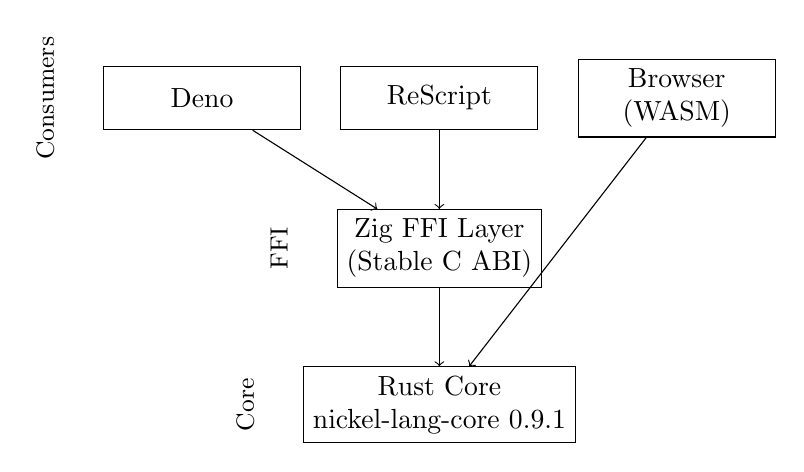
\begin{tikzpicture}[
    node distance=1.5cm,
    box/.style={rectangle, draw, minimum width=2.5cm, minimum height=0.8cm, align=center},
    layer/.style={rectangle, draw, dashed, inner sep=0.3cm},
]

% Consumer layer
\node[box] (deno) {Deno};
\node[box, right=0.5cm of deno] (rescript) {ReScript};
\node[box, right=0.5cm of rescript] (wasm) {Browser\\(WASM)};

% Zig layer
\node[box, below=1cm of rescript] (zig) {Zig FFI Layer\\(Stable C ABI)};

% Rust layer
\node[box, below=1cm of zig] (rust) {Rust Core\\nickel-lang-core 0.9.1};

% Arrows
\draw[->] (deno) -- (zig);
\draw[->] (rescript) -- (zig);
\draw[->] (wasm) -- (rust);
\draw[->] (zig) -- (rust);

% Layer labels
\node[left=0.5cm of deno, rotate=90, anchor=south] {\small Consumers};
\node[left=0.5cm of zig, rotate=90, anchor=south] {\small FFI};
\node[left=0.5cm of rust, rotate=90, anchor=south] {\small Core};

\end{tikzpicture}
\caption{Bunsenite three-layer architecture. Deno and ReScript access the Rust core through a Zig-provided stable C ABI. WebAssembly bindings connect directly via wasm-bindgen.}
\label{fig:architecture}
\end{figure}

\subsection{Layer 1: Rust Core}

The Rust core (\texttt{src/lib.rs}, \texttt{src/loader.rs}) provides the fundamental Nickel parsing and evaluation functionality:

\begin{lstlisting}[language=Rust,caption={Core NickelLoader implementation}]
pub struct NickelLoader {
    verbose: bool,
}

impl NickelLoader {
    pub fn parse_string(&self, source: &str, name: &str)
        -> Result<Value>
    {
        let mut program: Program<CBNCache> =
            Program::new_from_source(
                Cursor::new(source.as_bytes()),
                name,
                std::io::sink(),
            )?;

        let eval_result = program.eval_full()?;
        serde_json::to_value(&eval_result)
    }
}
\end{lstlisting}

The core enforces memory safety through Rust's ownership model. The \texttt{\#![deny(unsafe\_code)]} attribute ensures no unsafe blocks exist in the core library, with the single exception of the FFI boundary module.

\subsection{Layer 2: Zig FFI}

The Zig layer (\texttt{zig/bunsenite.zig}) provides a stable C ABI interface:

\begin{lstlisting}[language=C,caption={Zig FFI exports (C ABI)}]
// Import Rust FFI functions
extern fn bunsenite_parse(
    source: [*:0]const u8,
    name: [*:0]const u8
) callconv(.C) ?[*:0]u8;

// Re-export with stable names
pub export fn parse_nickel(
    source: [*:0]const u8,
    name: [*:0]const u8
) callconv(.C) ?[*:0]u8 {
    return bunsenite_parse(source, name);
}
\end{lstlisting}

This indirection provides several benefits:

\begin{enumerate}
    \item \textbf{ABI Isolation}: Consumer bindings depend on Zig's stable C ABI, not Rust's unstable ABI
    \item \textbf{Symbol Stability}: Function names and signatures remain constant across Rust compiler updates
    \item \textbf{Type Simplification}: Complex Rust types are converted to C-compatible primitives
\end{enumerate}

\subsection{Layer 3: Language Bindings}

\subsubsection{Deno Bindings}

Deno bindings use \texttt{Deno.dlopen} for native FFI:

\begin{lstlisting}[language=JavaScript,caption={Deno FFI binding}]
const symbols = {
  parse_nickel: {
    parameters: ["pointer", "pointer"],
    result: "pointer",
  },
  free_string: {
    parameters: ["pointer"],
    result: "void",
  },
};

const lib = Deno.dlopen(libPath, symbols);

export function parseNickel(source: string, name: string) {
  const resultPtr = lib.symbols.parse_nickel(
    toCString(source),
    toCString(name),
  );
  try {
    return JSON.parse(fromCString(resultPtr));
  } finally {
    lib.symbols.free_string(resultPtr);
  }
}
\end{lstlisting}

\subsubsection{ReScript Bindings}

ReScript bindings provide type-safe access with algebraic error handling:

\begin{lstlisting}[language=ML,caption={ReScript binding with Result type}]
type error =
  | ParseError(string)
  | ValidationError(string)
  | InvalidInput(string)

let parseNickel = (source: string, name: string)
    : result<Js.Json.t, error> => {
  let result = parseNickelRaw(source, name)
  switch Js.Nullable.toOption(result) {
  | Some(jsonString) => Ok(Js.Json.parseExn(jsonString))
  | None => Error(ParseError("Failed to parse: " ++ name))
  }
}
\end{lstlisting}

\subsubsection{WebAssembly Bindings}

For browser environments, Bunsenite compiles directly to WebAssembly using \texttt{wasm-bindgen}, bypassing the Zig layer since WASM provides its own stable binary interface.

\section{Safety Guarantees}

Bunsenite provides multiple layers of safety guarantees:

\subsection{Memory Safety}

\begin{itemize}
    \item \textbf{Rust Core}: Ownership and borrowing prevent use-after-free, double-free, and buffer overflows
    \item \textbf{FFI Boundary}: All FFI functions follow strict ownership protocols---callers receive owned pointers and must free them exactly once
    \item \textbf{Zig Layer}: No hidden allocations; all memory flows explicitly through the defined API
\end{itemize}

\subsection{Type Safety}

\begin{itemize}
    \item \textbf{Compile-time}: Rust's type system catches type errors before runtime
    \item \textbf{Binding-level}: ReScript's type system ensures correct usage in consuming code
    \item \textbf{Runtime}: Nickel's contract system validates configuration values
\end{itemize}

\subsection{Offline Operation}

Bunsenite has zero network dependencies in production code. This ``offline-first'' design ensures:

\begin{itemize}
    \item Operation in air-gapped environments
    \item No supply chain attacks via runtime network requests
    \item Deterministic behavior unaffected by network conditions
\end{itemize}

\section{Compliance and Standards}

Bunsenite adheres to the Rhodium Standard Repositories (RSR) framework at Bronze tier and the Trust Perimeter Classification Framework (TPCF) at Perimeter 3 (Community Sandbox).

\subsection{RSR Bronze Requirements}

\begin{table}[htbp]
\centering
\begin{tabular}{lll}
\toprule
\textbf{Requirement} & \textbf{Implementation} & \textbf{Verification} \\
\midrule
Type Safety & Rust compiler & Compile-time \\
Memory Safety & Ownership model & \texttt{\#![deny(unsafe\_code)]} \\
Offline-First & No network deps & Cargo audit \\
\bottomrule
\end{tabular}
\caption{RSR Bronze compliance matrix}
\label{tab:rsr}
\end{table}

\subsection{Security Considerations}

The library includes several security measures:

\begin{itemize}
    \item SHA-pinned dependencies in CI/CD workflows
    \item SPDX license headers on all source files
    \item Security policy with vulnerability reporting guidelines
    \item Automated security scanning via CodeQL and Dependabot
\end{itemize}

\section{Performance}

While a comprehensive performance evaluation is beyond the scope of this paper, preliminary benchmarks indicate:

\begin{itemize}
    \item \textbf{Parse latency}: Sub-millisecond for typical configuration files (<1KB)
    \item \textbf{FFI overhead}: Negligible (single function call indirection)
    \item \textbf{Memory usage}: Linear with configuration size
    \item \textbf{WASM size}: Optimized build produces ~2MB module
\end{itemize}

The three-layer architecture introduces minimal overhead because:

\begin{enumerate}
    \item Zig's FFI wrapper compiles to direct function calls
    \item JSON serialization happens once at the Rust layer
    \item Consumer bindings perform no additional parsing
\end{enumerate}

\section{Related Work}

\subsection{Configuration Languages}

Dhall~\cite{dhall} provides a programmable configuration language with strong normalization guarantees. CUE~\cite{cue} combines data validation with configuration. Unlike these, Nickel emphasizes gradual typing and seamless JSON interoperability.

\subsection{FFI Approaches}

Traditional approaches to multi-language FFI include:

\begin{itemize}
    \item \textbf{SWIG}: Generates bindings but requires complex configuration
    \item \textbf{Protocol Buffers}: Adds serialization overhead for simple cases
    \item \textbf{gRPC}: Introduces network complexity for local operations
\end{itemize}

Our Zig-based approach provides the simplicity of C FFI with the safety guarantees of a modern systems language.

\subsection{Rust FFI Libraries}

Libraries like \texttt{cbindgen} and \texttt{safer-ffi} help generate C headers from Rust code. Bunsenite's approach differs by introducing an explicit Zig layer for ABI stability, rather than relying on C header generation alone.

\section{Future Work}

Several extensions are planned:

\begin{itemize}
    \item \textbf{Language Server Protocol}: Integration with editors via tower-lsp
    \item \textbf{Watch Mode Optimization}: Incremental re-parsing for file watchers
    \item \textbf{Additional Bindings}: Python, Ruby, and JVM languages
    \item \textbf{Schema Generation}: Automatic JSON Schema from Nickel contracts
\end{itemize}

\section{Conclusion}

Bunsenite demonstrates that multi-language configuration parsing can be achieved without sacrificing memory safety or type guarantees. The three-layer architecture---Rust core, Zig FFI, language bindings---provides a template for building safe, stable, multi-language libraries.

The key insight is that Zig's C ABI compatibility, combined with Rust's memory safety, creates a sweet spot for FFI design: consumers get a stable interface while the implementation benefits from modern safety guarantees.

Bunsenite is open source under the MIT and Palimpsest-0.8 dual license, available at \url{https://github.com/hyperpolymath/bunsenite}.

\section*{Acknowledgments}

We thank the Nickel language team for nickel-lang-core, the Zig community for their work on C interoperability, and the Deno team for the excellent FFI API.

\bibliographystyle{plain}
\begin{thebibliography}{9}

\bibitem{nickel}
Tweag. \textit{Nickel: Better configuration for less}. \url{https://nickel-lang.org/}, 2024.

\bibitem{dhall}
Gabriel Gonzalez. \textit{Dhall: A programmable configuration language}. \url{https://dhall-lang.org/}, 2024.

\bibitem{cue}
Marcel van Lohuizen. \textit{CUE: Configure Unify Execute}. \url{https://cuelang.org/}, 2024.

\bibitem{rust-abi}
Rust Language Team. \textit{The Rust Reference: Type Layout}. \url{https://doc.rust-lang.org/reference/type-layout.html}, 2024.

\bibitem{zig-ffi}
Andrew Kelley et al. \textit{Zig Language Reference: C Interoperability}. \url{https://ziglang.org/documentation/master/}, 2024.

\bibitem{wasm-bindgen}
The Rust and WebAssembly Working Group. \textit{wasm-bindgen Guide}. \url{https://rustwasm.github.io/wasm-bindgen/}, 2024.

\bibitem{deno-ffi}
Deno Land Inc. \textit{Deno FFI}. \url{https://deno.land/manual/runtime/ffi_api}, 2024.

\end{thebibliography}

\end{document}
